\chapter{\Large Visualization Recommendation for Incremental Data based on Intent (IVR\_I)}


Our proposed approach is discussed to handle the incremental data that has been generated over time in the real world. Nowadays, data is growing tremendously in an incremental fashion. The data can be added in terms of volume in big data in a dynamic environment horizontally (instances are added) or/and vertically (new dimensions are added). It is quite challenging to provide the visualization recommendation in this situation and the problem remained unaddressed. There are many approaches for recommending the visualization for entire data (existing and incremental data) but they are time consuming and very expensive because considering the entire data from the scratch and repeating this procedure. To address this issue, our approach recommends the visualization for entire data by executing the recommendation algorithm exclusively on incremental data which saves the time. 

Intent Aware Visualization Recommendation (IAVR) algorithm \cite{maruta2021intent} is applied to existing data and intent which will generate visualization type and visualized columns. Over the period the same algorithm \cite{maruta2021intent} is applied exclusively on incremental data and intent, which provides visualization type and visualized columns for incremental data. The obtained visualization types and visualized columns for existing and incremental data are compared. The visualization type will be varying for the vertical increments of the data where the added dimension names are part of the intent. In this paper we addressed only when both the results (visualization type and visualized columns) are the same and recommended the visualization for the entire data (existing and incremental data) without carrying the experiments from the scratch and it is very less time consuming. If the results are not the same either of the results are recommended for the entire data (existing and incremental data). If the visualization type is bivariate, then plot a bivariate visualization for the top two set of visualized columns. If the visualization type is not bivariate, then plot a univariate visualization for the top single visualized column. Fig.~\ref{fig1} will summarize our proposed strategy.



\begin{figure}[h]
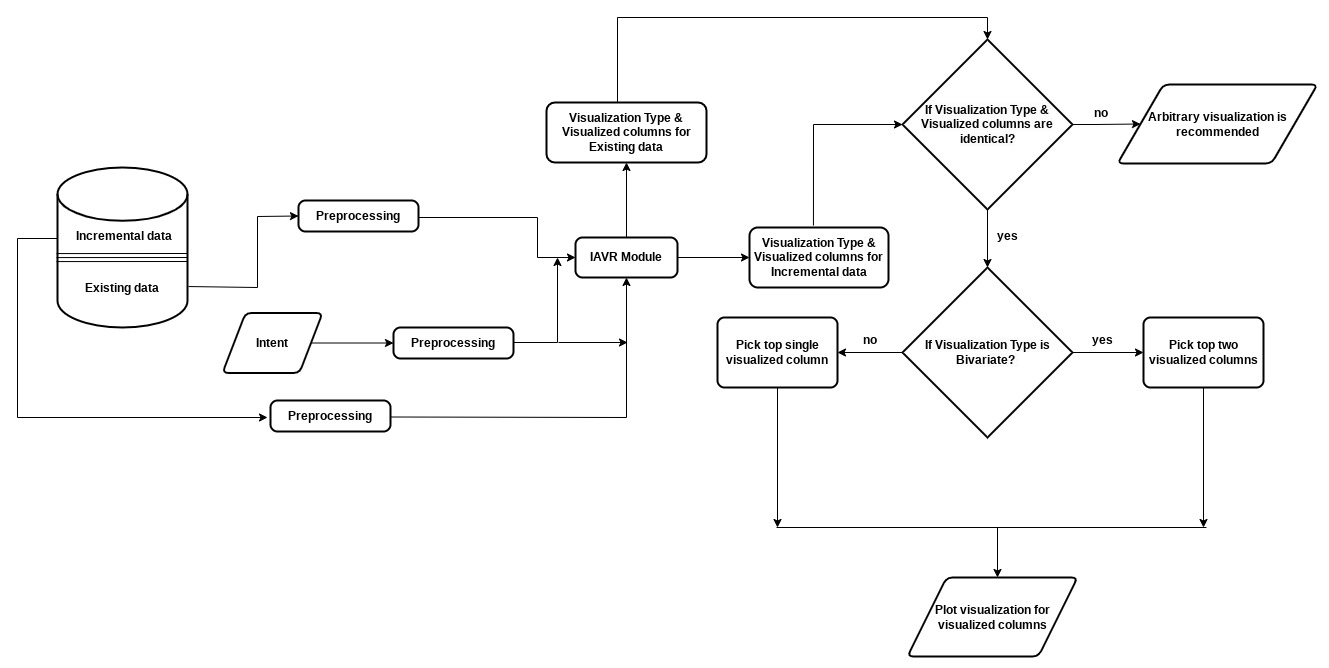
\includegraphics[width=\textwidth]{IVRIimages/flow (2).jpg}
\caption{Workflow of IVR} \label{fig1}
\end{figure}

\section{Workflow Description}

\subsection{Preprocessing:} The benchmark datasets are to be preprocessed where the missing values are replaced by median of the remaining values when the values are numeric, in other case when the data value is a string, it will be replaced with the repeated string. In addition the null values and the duplicate instances in the dataset are also removed. The preprocessed dataset is converted into the JSON format for further processing.
\subsection{Intent:} User requests are formally placed in simple sentences to visualize the data which is termed as Intent. For example Region wise insurance analysis is used as intent to obtain analysis region wise for Prediction of Insurance Charges dataset. Maruto et.al., \cite{maruta2021intent} have taken the intent as title of each visualization in a specific dataset which was crawled from Tableau public web. In our approach we analyzed the dataset and obtained the suitable intents for different datasets.
\subsection{Preprocessing Intent:} The intent is also preprocessed by removing the stop words. The words in the intent are also mapped with synonyms which could give more accurate results. The preprocessed intent is added to the dataset which is JSON format.
\subsection{Incremental dataset:} There could be two possible increments for the dataset. The increments could be instances added to the existing data which we termed as horizontal increments and adding dimensions to the existing data which we termed as vertical increments. Here we considered all possible horizontal increments and vertical increments 10\% , 20\%  till 50\% of the data size and the number of dimensions respectively. Further, the preprocessing of incremental data is also done.

\subsection{IAVR Module} 

Maruta et.al.,\cite{maruta2021intent} have proposed a visualization recommendation approach where the intent and dataset are taken as input and outputs the visualization type (Bar chart, Line chart, Pie chart etc.,), visualized columns (percentage that each column in the dataset can be part of visualization). They have used BiDA \cite{seo2016bidirectional} and BERT \cite{devlin2018bert} models for predicting the visualization type and visualized columns. Visualization type is predicted by providing both the intent embedding and the column embedding in the dataset to the BiDA model. The output of the BiDA model is given to the multilayer perceptron and softmax function is used to finally predict the visualization type. For extracting the visualized columns the intent and dataset headers are given to the pretrained BERT model. The output of the BERT model is combined with statistical features of the attributes of the dataset in order to obtain the probability of each column that could be visualized.

\begin{algorithm}[!ht]
\caption{Incremental Visualization Recommendation (IVR)}\label{algo1}
\KwIn{ Dataset (D),  Intent (I)}
\KwOut{Visualization (V)}
Preprocess D \& I

\(EV \leftarrow IAVR(D,I)\)

\If{hy = 1 and vy = 0}
{
\(IV \leftarrow IAVR(hy,I)\)
}   
\ElseIf{vy = 1 and hy = 0}
{
    \(IV \leftarrow IAVR(vy,I)\)
}
\ElseIf{vy = 1 and hy = 1}
{
    \(IV \leftarrow IAVR(hy+vy,I)\)
}
\If{EV = IV}
{
    \If{VT = 1}
    {
        \(VC \leftarrow (VC0,VC1)\)
    }
    \Else
    {    
    \(VC \leftarrow (VC0)\)
    }
}
    \(V \leftarrow plot(VT, VC)\)
    
\KwRet{V}
\end{algorithm}
\section{Algorithm Description}
The dataset and intent are taken as input. Preprocessing of the dataset and intent is done which was discussed earlier in section 3.1. Incremental data is added to the dataset horizontally (hy) and vertically (vy). hy and vy can take the value either 0 or 1 where 1 indicates increments and 0 indicates no increments. IAVR is an Intent Aware Visualization Recommendation algorithm \cite{maruta2021intent} which will give visualization (visualization type and visualized columns)  as output. IAVR is applied for existing data (D) and Intent (I) which will give a visualization recommendation and it is  termed as Existing Visualization (EV). When the data is evolving in a data stream, then IAVR \cite{maruta2021intent} is applied to the chunks of incremental data without considering the data from scratch. Ultimately, we will get a visualization recommendation exclusively for incremental data and termed as Incremental Visualization (IV). Now EV and IV recommendations are compared if both are same then visualization type (VT) is checked. VT can take the value either 0 or 1 where 1 indicates bivariate and 0 indicates univariate. If the visualization type is bivariate the top two visualized columns (VC) are chosen (VC0 \& VC1) otherwise the top visualized column is chosen (VC0). Finally visualization is plotted for the visualized columns (VC) based on visualization type (VT).




\section{Comparison between traditional and proposed approach}

\begin{table}[H]
\caption{Comparison of our proposed approach with traditional approach}\label{tab1}
\scalebox{0.56}
{
\begin{tabular}{|c|c|}
\hline
\textbf{Traditional Maruto et.al., (2021) \cite{maruta2021intent}} &  \textbf{Proposed Approach IVR}\\
\hline
Can’t handle incremental data & Handles incremental data\\
\hline
Used synthetic dataset &  Used benchmark datasets \\
\hline
Can’t handle volume and velocity in the context of data of big data & Handles volume and velocity in the context of data of big data\\
\hline
Time consuming & Less time consuming\\
\hline
\end{tabular}
}
\end{table}







\section{Discussions and Experimental results}
Experiments performed for three standard benchmark datasets of the Kaggle database i.e Prediction of Insurance Charges, AQI - Air Quality Index, California House Price. All of these datasets have different data sizes and dimensions.
We generated intents from each dataset to perform experiments and the details are provided. Later, the dataset is divided into two parts in the ratio of (90:10, 80:20, 70:30, 60:40, 50:50). First part is considered as existing data and the remaining part is considered as incremental data (it can be horizontal and vertical increments).
A pre-trained GloVe model \cite{pennington2014glove} is used for word embedding. This model was trained using the Wikipedia 2014 dump and Gigaword 5 corpus. For predicting the visualization type BiDA model is used with six layers in the multilayer perceptron \cite{maruta2021intent}. For identifying visualized columns a pre-trained BERT model is used with two layers in the multilayer perceptron \cite{maruta2021intent}. 
\subsection{Experimental Results} 
The IAVR \cite{maruta2021intent} algorithm is applied to the first part treating as existing data and obtaining the desired results. Then same algorithm is applied to the second part treating as incremental data. Comparing the visualization results (VT and VC) and recommend the visualization for the entire data (existing and incremental data). Hence, IAVR \cite{maruta2021intent} is applied for every timestamp for incremental data and recommends visualization for the entire data (existing and incremental data). 
Table 2 shows the results obtained with our proposed approach.


\begin{table}[ht]
\caption{Experimentation of our proposed approach with benchmark datasets for horizontal and vertical increments}\label{tab2}
\scalebox{0.8}{\renewcommand{\arraystretch}{2.5}
\begin{tabular}{|p{3cm}|p{3cm}|p{3cm}|p{3cm}|p{3cm}|}
\hline
\textbf{Dataset} & \textbf{Intent} & \textbf{Incremental data (Horizontal and Vertical)} & \textbf{Visualization recommendation for existing data}  & \textbf{Visualization recommendation for incremental data}       \\ \hline
\multirow{2}{*}{\parbox{3cm}{Prediction of Insurance Charges Size: 1337 X 5}} & Region wise insurance analysis & \multirow{2}{*}{\parbox{3cm}{10\%, 20\%, 30\%, 40\% and 50\% of data size and number of dimensions respectively.}} & Pie Chart for region column & Pie Chart for region column  \\
 \cline{2-2} \cline{4-5}  
 & Impact of insurance charges on having children &  & Bar Chart between having children and insurance charges & Bar Chart between having children and insurance charges
 
 \\
 \hline
\multirow{2}{*}{\parbox{3cm}{AQI - Air Quality Index\\ Size:\\ 10127 X 4}} & Air Quality Index value according to country & \multirow{2}{*}{\parbox{3cm}{10\%, 20\%, 30\%, 40\% and 50\% of data size and number of dimensions respectively.}} & Line Chart between AQI value and country & Line Chart between AQI value and country  \\
\cline{2-2} \cline{4-5}
 & Examination of population close to ocean & & Bar Chart between ocean proximity and population & Bar Chart between ocean proximity and population \tabularnewline
 \hline
\multirow{2}{*}{\parbox{3cm}{California House Price\\ Size:\\ 20640 X 10}} & House value effect on  number of bedrooms & \multirow{2}{*}{\parbox{3cm}{10\%, 20\%, 30\%, 40\% and 50\% of data size and number of dimensions respectively.}} & Bar Chart between median house value and total bedrooms & Bar Chart between median house value and total bedrooms \\
\cline{2-2} \cline{4-5}      
 & Examination of population close to ocean  &  & Bar Chart between ocean proximity and population & Bar Chart between ocean proximity and population\tabularnewline
 \hline
\end{tabular}}
\end{table}



The above tabulated results show that the visualization recommendation for the existing data and incremental data (horizontal and vertical) are the same. Hence that particular visualization is recommended for the entire data (existing and incremental data).
\subsection{Analysis of the results }
Experimentation done on the benchmark Air Quality Dataset by considering the range from 2000 instances till 10000 instances in an incremental fashion and we have observed that our proposed (incremental) approach has taken considerably less time than the traditional approach  which is depicted in Fig.~\ref{fig3}.

\begin{figure}[ht]
\centering
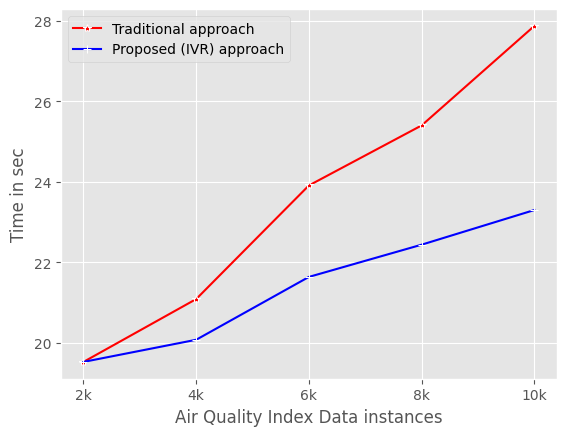
\includegraphics[height=5cm,width=9cm]{IVRIimages/time (2).png}
\caption{Workflow of IVR} \label{fig3}
\end{figure}


In our experimentation we have considered two cases to analyze the results. When the instances are added to the existing data those are considered as horizontal increments which we categorized as Case 1 and dimensions are added to the existing data those are considered as vertical increments which we categorized as Case 2.\\
\textbf{Case 1:}\\
When horizontal increments are added to the data, the visualization recommendation by our approach is the same for the existing and incremental data.\\
\textbf{Case 2:}\\
There are again two phases with vertical increments.
\begin{itemize}
    \item The added dimension names are not part of the intent 
    \item The added dimension names are part of the intent
\end{itemize}

When the added dimension names are not part of the intent, the visualization recommendation by our approach is the same for the existing and incremental data. When the dimension names are part of the intent, we observed that in some cases the visualization recommendation for existing and incremental data is different then arbitrary visualization recommendation is suggested. The details of this work are in progress but beyond the scope of this paper.